\section{Global Comparison and Discussion}

The inter-model comparison presented in this section is based exclusively on the \texttt{tuned} variants evaluated through nested cross-validation. This choice limits the selection bias introduced by hyperparameter tuning, in accordance with established recommendations in the model-evaluation literature (Varma and Simon, 2006; Cawley and Talbot, 2010). The untuned variants and model-specific diagnostics retain an interpretive role, while the frozen corroboration set remains a secondary control.

\subsection{Confirmatory Inter-Model Results}
The following table compares the six model families on the basis of their confirmatory \texttt{tuned} performance, with \texttt{macro-F1} as the primary metric and \texttt{accuracy} as the secondary metric.

\begin{table}[H]
\centering
\begin{tabular}{|l|r|r|r|}
\hline
\textbf{Model} & \textbf{Macro-F1 (mean $\pm$ std)} & \textbf{Accuracy (mean $\pm$ std)} & \textbf{Time (s)} \\
\hline
Logistic regression & $0.9787 \pm 0.0198$ & $0.9848 \pm 0.0146$ & \texttt{77.05} \\
RBF SVM & $0.9756 \pm 0.0207$ & $0.9823 \pm 0.0151$ & \texttt{56.49} \\
Random forest & $0.9702 \pm 0.0140$ & $0.9747 \pm 0.0089$ & \texttt{250.11} \\
MLP & $0.9389 \pm 0.0322$ & $0.9482 \pm 0.0279$ & \texttt{38.25} \\
Perceptron & $0.8085 \pm 0.0523$ & $0.8409 \pm 0.0411$ & \texttt{29.79} \\
Decision tree & $0.4295 \pm 0.0546$ & $0.4610 \pm 0.0627$ & \texttt{11.47} \\
\hline
\end{tabular}
\caption{Confirmatory inter-model comparison}
\end{table}

\begin{figure}[H]
\centering
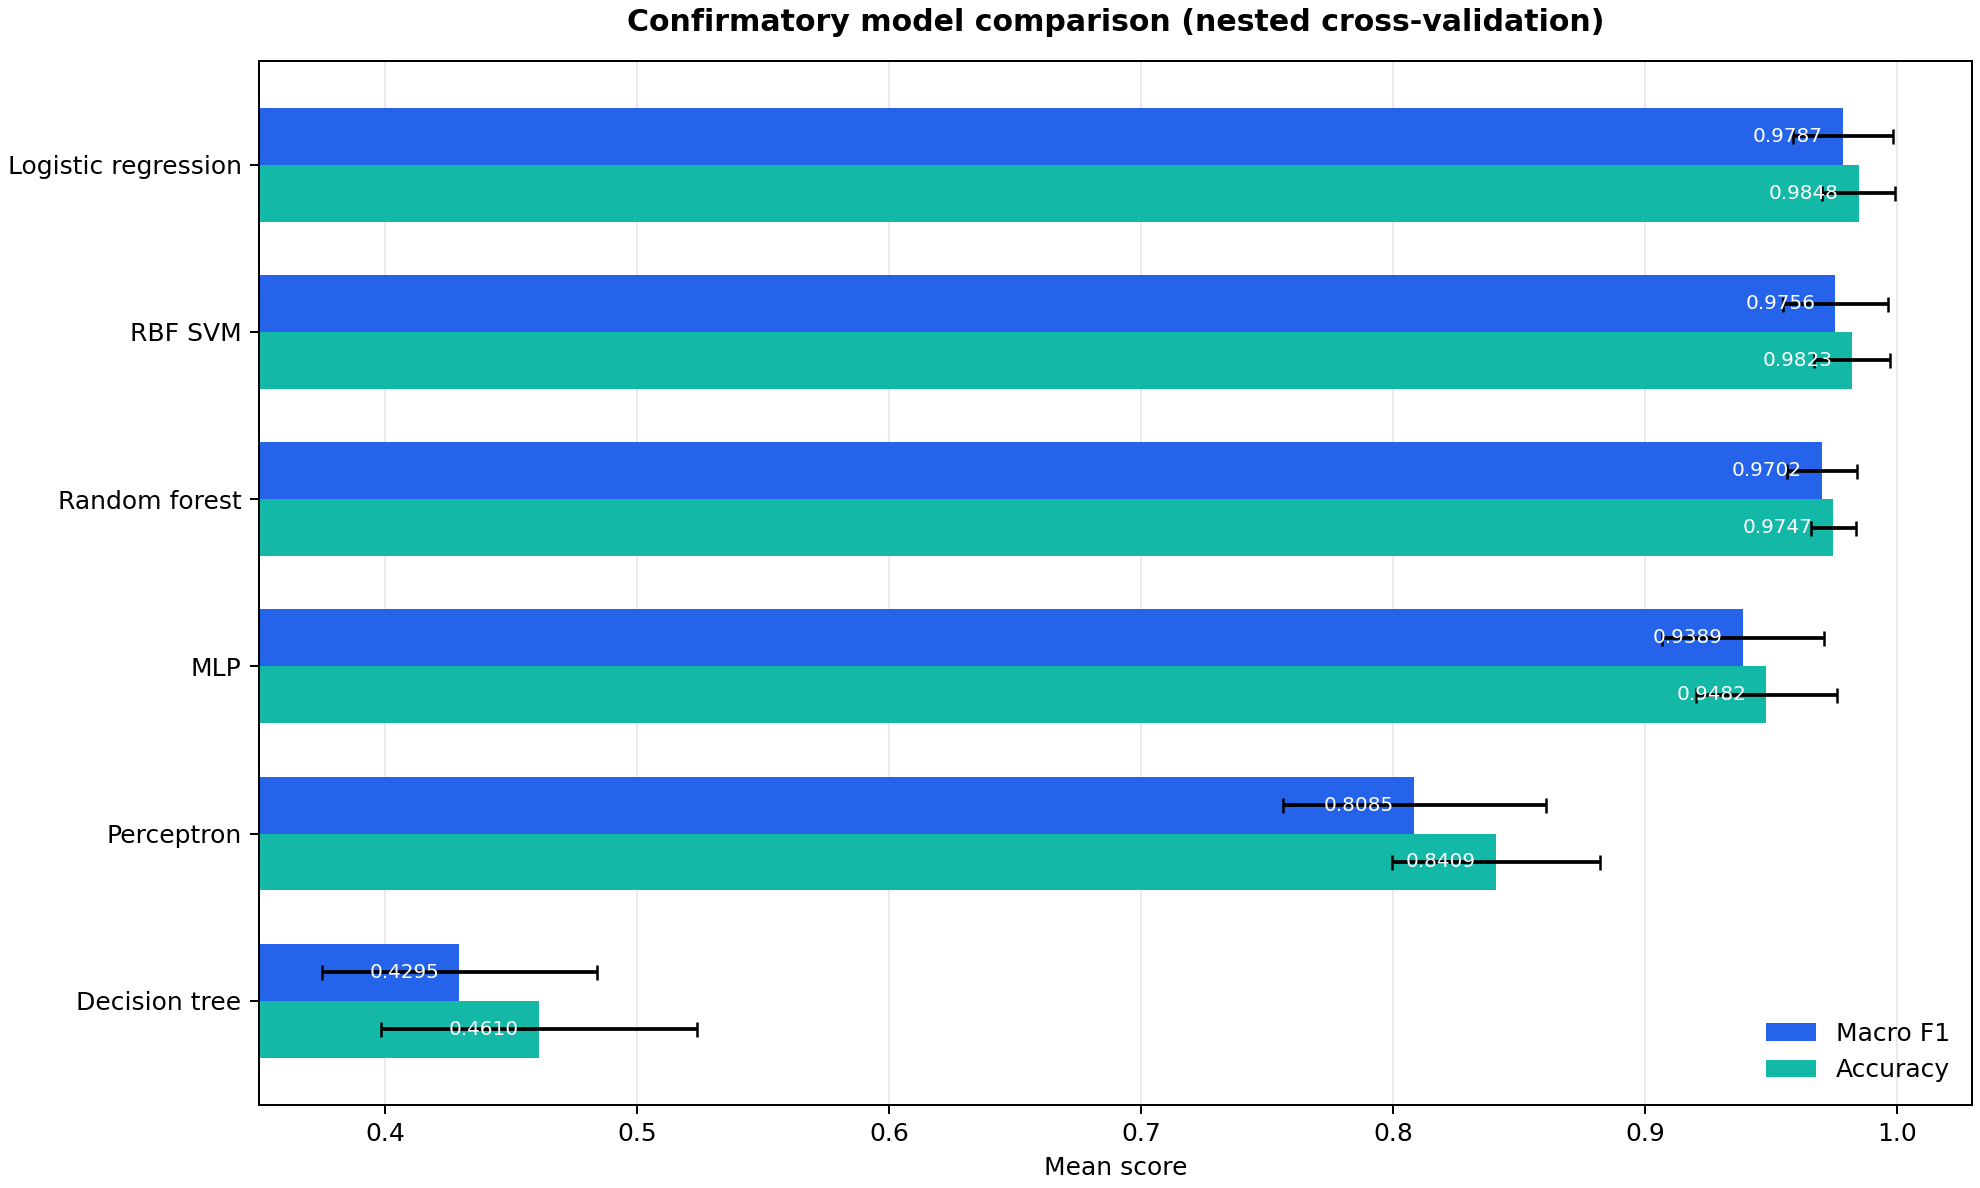
\includegraphics[width=\textwidth]{../figures/en/fig02_barplot_comparatif_tuned.png}
\caption{Confirmatory inter-model comparison}
\end{figure}

A clear hierarchy emerges. Logistic regression and the RBF SVM form the leading confirmatory pair, with a slight average advantage for logistic regression. The random forest also performs at a very high level, although it falls slightly behind. The MLP is a credible solution but does not match the top three models. The perceptron serves effectively as a linear baseline after preprocessing, whereas a single decision tree is clearly inadequate for this multiclass problem.

The key point is the proximity of logistic regression and the SVM. Their mean \texttt{macro-F1} scores differ only slightly, although logistic regression retains the higher average. In the absence of a formal statistical test between these closely matched models, it is more prudent to describe them as confirmatory co-leaders, with logistic regression leading on the mean, than to claim a single definitive winner.

\subsection{Relative Stability and Practical Trade-offs}
Cross-fold standard deviations do not constitute a statistical test, but they provide useful information about the relative stability of the model families under the selected protocol.

\begin{table}[H]
\centering
\begin{tabular}{|l|r|l|}
\hline
\textbf{Model} & \textbf{F1 range} & \textbf{Stability assessment} \\
\hline
Logistic regression & \texttt{0.0512} & Very good stability \\
RBF SVM & \texttt{0.0549} & Stability comparable to logistic regression \\
Random forest & \texttt{0.0343} & Most stable of the three leading models \\
MLP & \texttt{0.0896} & More pronounced variability \\
Perceptron & \texttt{0.1121} & Insufficient stability for a leading position \\
Decision tree & \texttt{0.1449} & Very high structural instability \\
\hline
\end{tabular}
\end{table}

\begin{figure}[H]
\centering
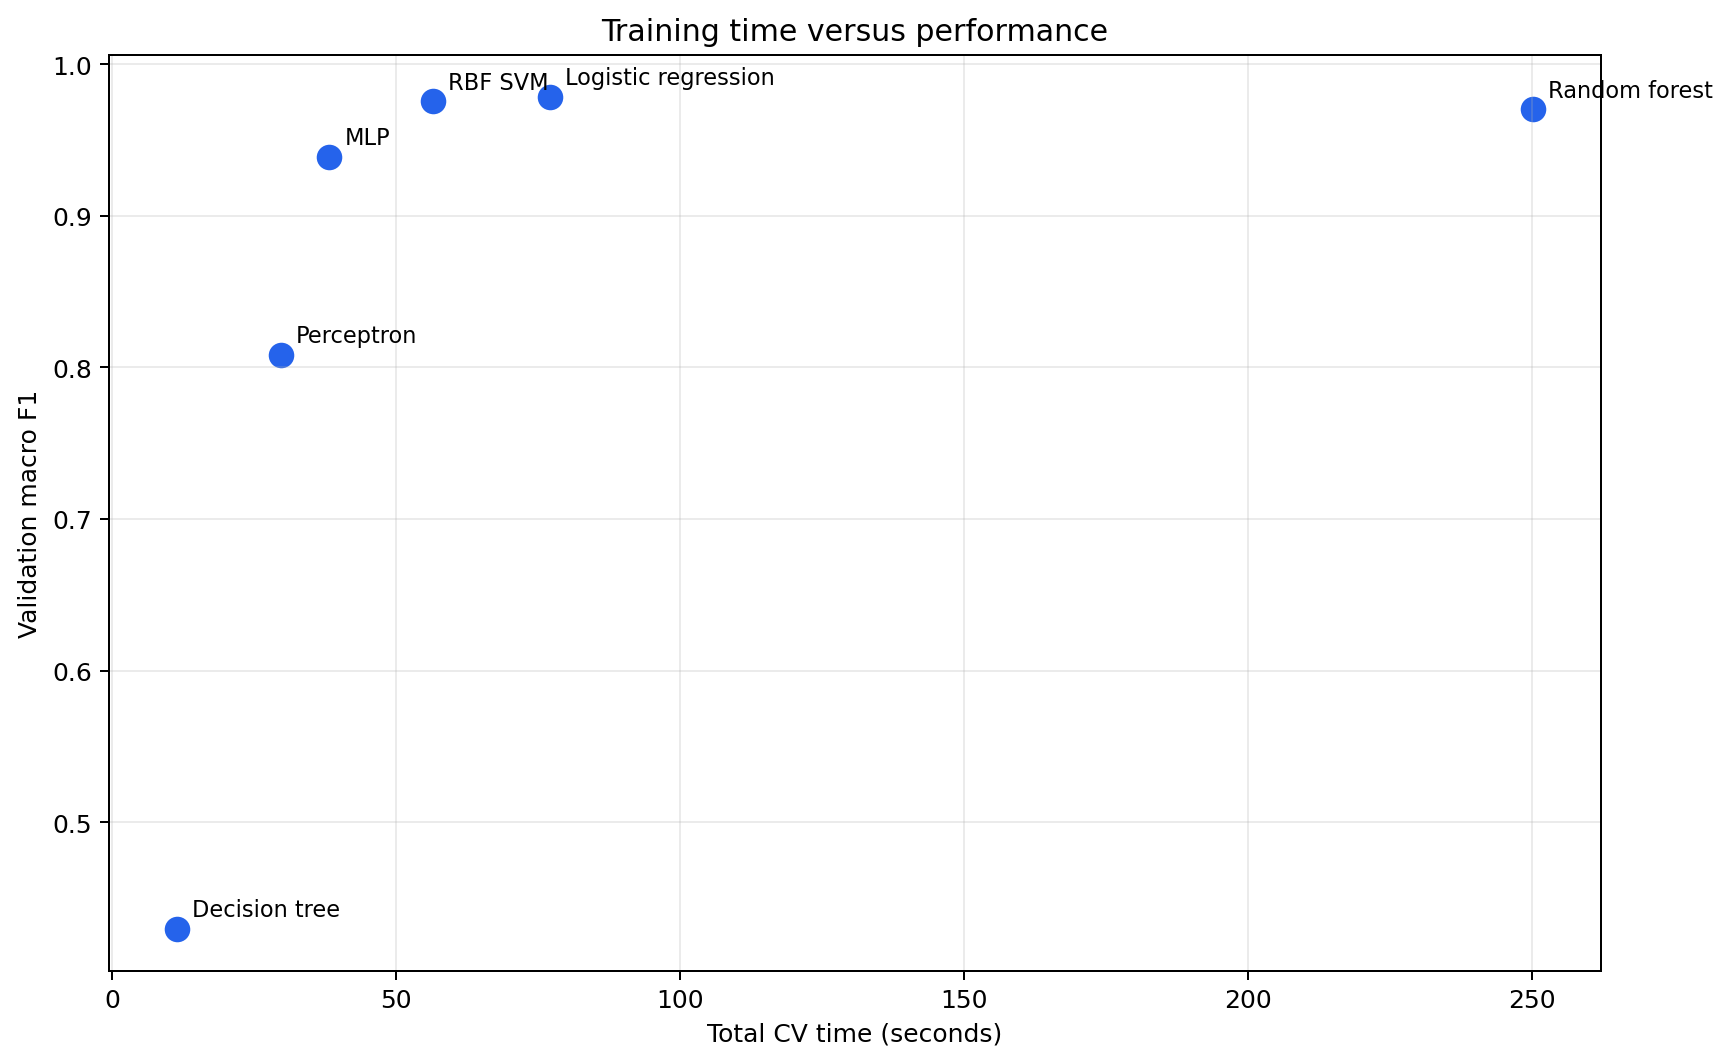
\includegraphics[width=\textwidth]{../figures/en/fig3b_temps_vs_performance.png}
\caption{Compute-time/performance trade-off}
\end{figure}

From a practical standpoint, logistic regression offers the best balance of average performance, computational cost, and interpretability. It achieves the highest observed confirmatory performance while remaining easier to interpret than an RBF SVM and far less expensive than a random forest. The SVM produces a very similar result, but with lower interpretability. The random forest confirms its robustness, although its computational cost is by far the highest among the leading models.

The MLP and perceptron are relatively fast, but that advantage does not offset their performance deficit relative to the strongest candidates. Finally, although the decision tree is inexpensive, its weak predictive performance prevents it from being a defensible solution for this project.

\subsection{Cross-Model Error Analysis}
The \texttt{tuned} OOF predictions on the development subset (\texttt{n = 792}) complement the overall analysis with a more detailed view of the number and profile of errors.

\begin{table}[H]
\centering
\begin{tabular}{|l|r|r|r|}
\hline
\textbf{Model} & \textbf{Correct predictions} & \textbf{Errors} & \textbf{Error rate} \\
\hline
Logistic regression & \texttt{780} & \texttt{12} & \texttt{1.5 \%} \\
RBF SVM & \texttt{778} & \texttt{14} & \texttt{1.8 \%} \\
Random forest & \texttt{772} & \texttt{20} & \texttt{2.5 \%} \\
MLP & \texttt{751} & \texttt{41} & \texttt{5.2 \%} \\
Perceptron & \texttt{666} & \texttt{126} & \texttt{15.9 \%} \\
Decision tree & \texttt{365} & \texttt{427} & \texttt{53.9 \%} \\
\hline
\end{tabular}
\end{table}

This perspective confirms the hierarchy observed for \texttt{macro-F1}. The two co-leaders make very few errors across the development set, the random forest remains close behind, and a more substantial gap then appears before the MLP, perceptron, and especially the decision tree. In other words, the difference between the strongest and weaker models is not limited to small score fluctuations: it corresponds to a change in the order of magnitude of the error count.

The overlap among the errors made by the three strongest models provides further insight.

\begin{table}[H]
\centering
\begin{tabular}{|l|r|r|r|}
\hline
\textbf{Comparison} & \textbf{Shared errors} & \textbf{Error union} & \textbf{Jaccard} \\
\hline
Logistic regression vs.\ SVM & \texttt{10} & \texttt{16} & \texttt{0.625} \\
Logistic regression vs.\ random forest & \texttt{5} & \texttt{27} & \texttt{0.185} \\
SVM vs.\ random forest & \texttt{5} & \texttt{29} & \texttt{0.172} \\
\hline
\end{tabular}
\end{table}

Logistic regression and the SVM therefore share a substantial portion of their residual errors. The overlap is high: 10 shared errors out of 16 distinct errors in total, yielding a Jaccard index of \texttt{0.625}. This proximity is consistent with their nearly identical performance and suggests that they exploit very similar discriminative structures. The random forest shares fewer errors with either model, supporting the idea that it has a partially different error profile without altering its slight disadvantage on the primary metric.

Overall, the cross-model error analysis suggests that the remaining gains no longer depend on coarse global separation, but on a small number of ambiguous cases. The strongest models therefore differ less in how they represent the general nature of the problem than in their ability to handle these residual decision-boundary regions.

\subsection{Secondary Corroboration on the Frozen Set}
The frozen corroboration set provides a secondary external check of the selected pipelines. It replaces neither the confirmatory logic of \texttt{nested CV} nor the hierarchy established above.

\begin{table}[H]
\centering
\begin{tabularx}{\textwidth}{|>{\raggedright\arraybackslash}p{3.0cm}|>{\centering\arraybackslash}p{2.8cm}|>{\centering\arraybackslash}p{2.2cm}|>{\centering\arraybackslash}p{2.2cm}|Y|}
\hline
\textbf{Model} & \textbf{Reference variant} & \textbf{Reference corroboration F1} & \textbf{Tuned corroboration F1} & \textbf{Assessment} \\
\hline
Logistic regression & \texttt{scaled\_only} & \texttt{0.9892} & \texttt{0.9892} & Neutral tuning effect on corroboration \\
RBF SVM & \texttt{scaled\_only} & \texttt{0.9838} & \texttt{0.9946} & Favorable tuning effect on corroboration \\
Random forest & \texttt{default} & \texttt{0.9842} & \texttt{0.9842} & Neutral tuning effect on corroboration \\
MLP & \texttt{scaled\_only} & \texttt{0.9785} & \texttt{0.9785} & Neutral tuning effect on corroboration \\
Perceptron & \texttt{scaled\_only} & \texttt{0.8815} & \texttt{0.8694} & Slightly unfavorable tuning effect on corroboration \\
\hline
\end{tabularx}
\end{table}

\begin{figure}[H]
\centering
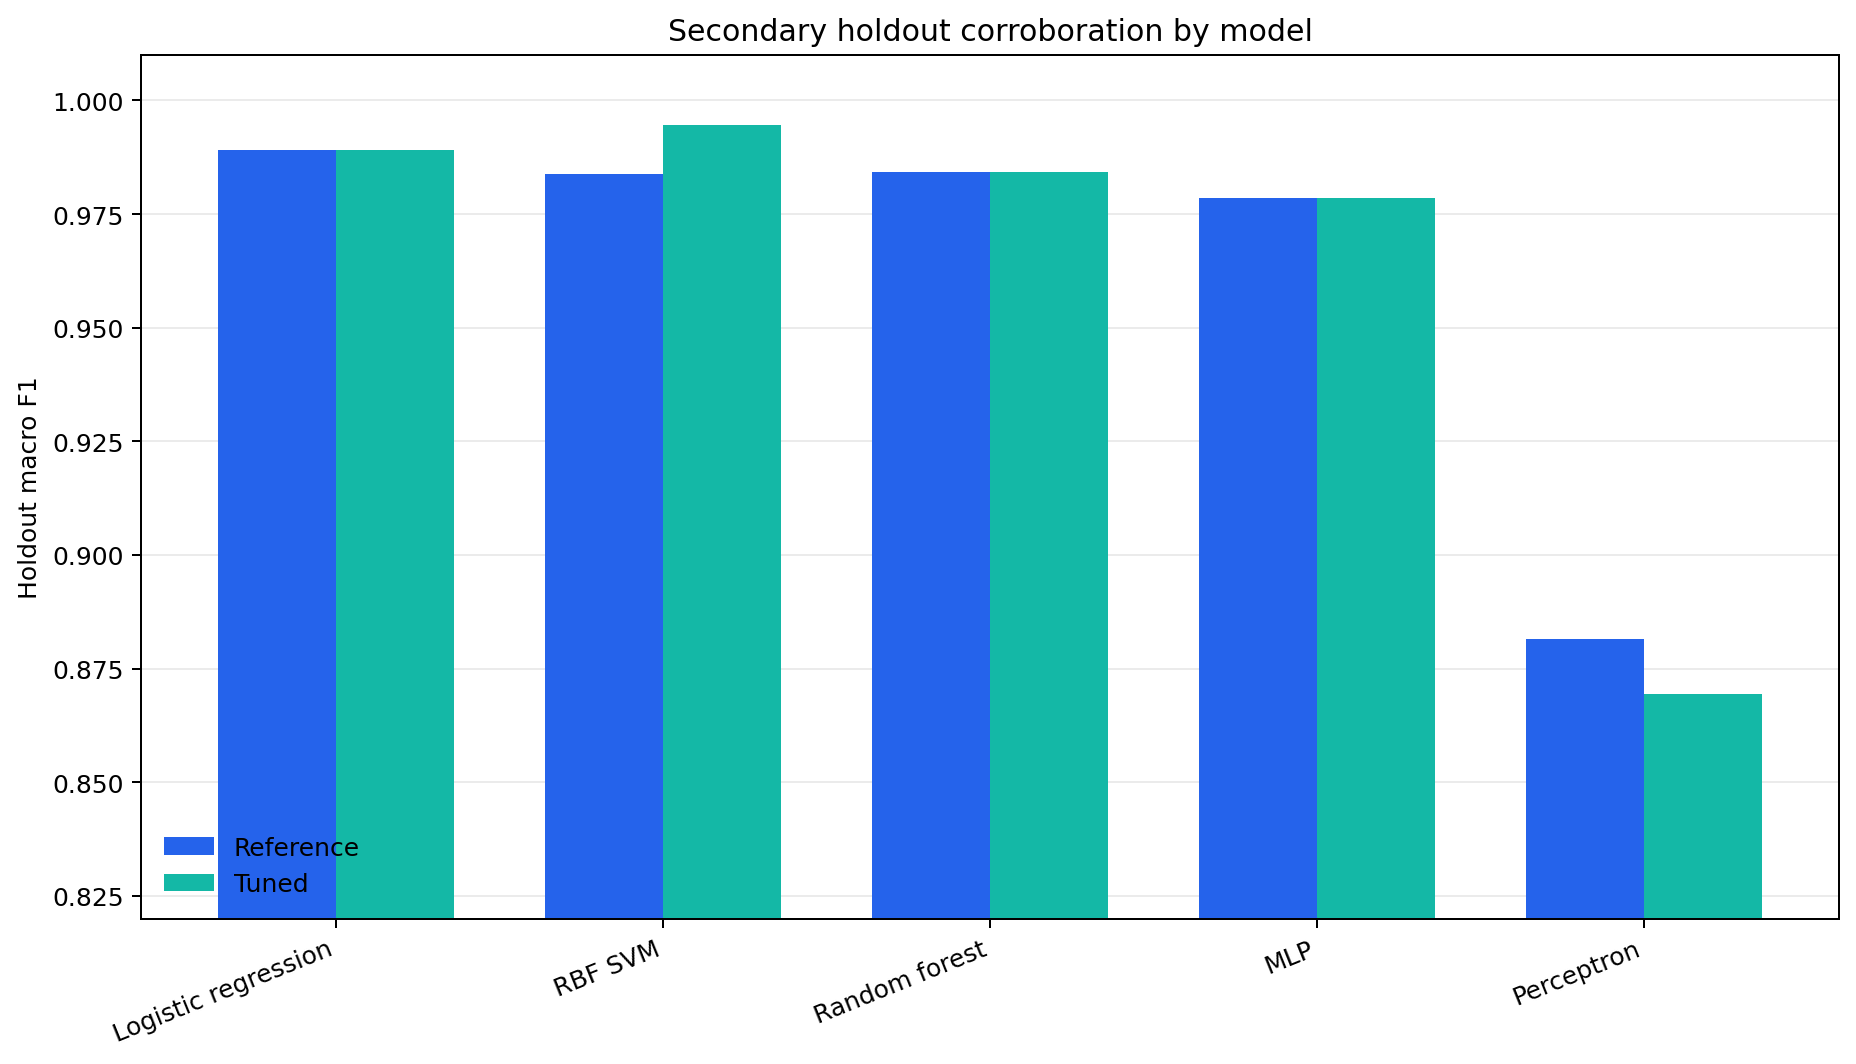
\includegraphics[width=\textwidth]{../figures/en/fig_global_corroboration_holdout.png}
\caption{For each eligible model, comparison of the reference variant selected on the development set with the \texttt{tuned} variant on the frozen corroboration set.}
\end{figure}

Considered in isolation, these figures might suggest reranking some models. Such an interpretation would be methodologically unsound. The corroboration set does not represent a new selection stage here, but rather a final secondary check on a single split. It broadly confirms the strength of the leading pipelines, but it should not be used to overturn the primary hierarchy based on confirmatory nested cross-validation estimates.

\subsection{Scientific Discussion}
Several general lessons emerge from the study. First, a well-regularized linear model can remain extremely competitive in a high-dimensional multiclass problem when paired with suitable preprocessing. Logistic regression shows that a relatively parsimonious structure can be sufficient to achieve a very high level of generalization.

Second, the RBF SVM confirms the presence of exploitable nonlinear structure, but provides no measurable improvement over logistic regression. In this context, practical criteria---particularly interpretability and computational cost---can therefore guide the choice between the two.

Third, the random forest also warrants attention. Its very strong performance without scaling shows that an aggregated tree-based approach can capture the problem structure effectively. However, its substantial additional cost and slight deficit in \texttt{macro-F1} make it a less natural choice when the objective is the best overall trade-off.

The MLP results are also instructive. The model becomes competitive after normalization, but it does not outperform the strongest, simpler approaches. This observation is consistent with a dataset that is relatively modest in size given the multiclass complexity of the problem: greater representational capacity does not automatically yield better generalization.

Finally, the contrast between the decision tree and random forest underscores the decisive role of aggregation. The interpretability of a single tree is not enough when the model's variance becomes excessive. Here, the individual tree primarily serves as a useful counterpoint that illustrates what the ensemble corrects.

In summary, the project demonstrates above all that a well-regularized linear model can remain highly competitive when supported by appropriate preprocessing. The gains from more flexible models are modest here and must be assessed in light of their cost, stability, and interpretability.

% ==========================================
% 5. CONCLUSION
% ==========================================
